\documentclass[border=8pt]{standalone}
\usepackage{amsmath,amssymb}
\usepackage{tikz}
\usetikzlibrary{arrows.meta,calc,decorations.pathreplacing,decorations.pathmorphing,patterns,shapes.geometric,positioning,shadings,plotmarks}

\begin{document}
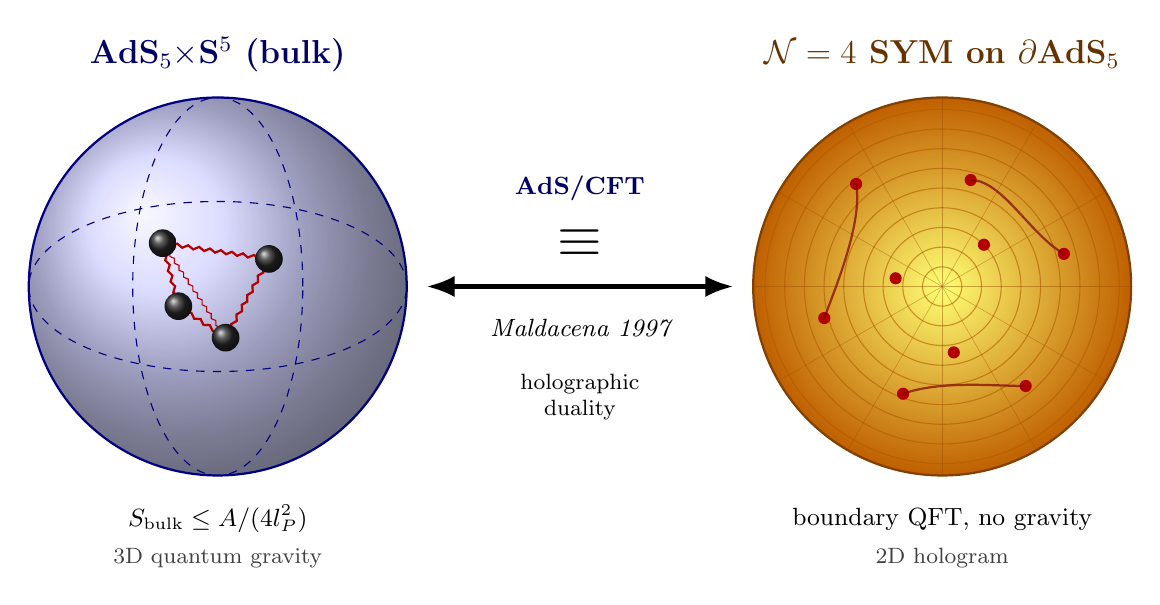
\begin{tikzpicture}[>=Latex]

% =========================================================
% LEFT PANEL: 3D bulk volume with particles
% =========================================================
\def\leftCx{-4.6}
\def\leftCy{0}
\def\R{2.4}

% Bulk sphere (3D look) using ball shading
\shade[ball color=blue!22,opacity=0.85] (\leftCx,\leftCy) circle (\R);
\draw[blue!50!black,thick] (\leftCx,\leftCy) circle (\R);

% Equator ellipse (give 3D feel)
\draw[blue!50!black,dashed,thin] (\leftCx,\leftCy) ellipse ({\R} and {0.45*\R});

% Vertical great circle suggestion
\draw[blue!50!black,dashed,thin] (\leftCx,\leftCy) ellipse ({0.45*\R} and {\R});

% Particles inside bulk (small filled balls)
\coordinate (P1) at ($(\leftCx,\leftCy)+(-0.7,0.55)$);
\coordinate (P2) at ($(\leftCx,\leftCy)+(0.65,0.35)$);
\coordinate (P3) at ($(\leftCx,\leftCy)+(0.10,-0.65)$);
\coordinate (P4) at ($(\leftCx,\leftCy)+(-0.50,-0.25)$);

% Field/string lines connecting particles (gravitational/gauge interactions)
\draw[red!70!black,thick,decorate,decoration={snake,amplitude=0.6pt,segment length=4pt}] (P1) -- (P2);
\draw[red!70!black,thick,decorate,decoration={snake,amplitude=0.6pt,segment length=4pt}] (P2) -- (P3);
\draw[red!70!black,thick,decorate,decoration={snake,amplitude=0.6pt,segment length=4pt}] (P3) -- (P4);
\draw[red!70!black,thick,decorate,decoration={snake,amplitude=0.6pt,segment length=4pt}] (P4) -- (P1);
\draw[red!70!black,thin,decorate,decoration={snake,amplitude=0.5pt,segment length=3pt}] (P1) -- (P3);

% Particles on top
\foreach \p in {P1,P2,P3,P4} {
  \shade[ball color=black!85] (\p) circle (5pt);
}

% Top label
\node[font=\large\bfseries,blue!40!black] at (\leftCx,\leftCy+\R+0.55) {AdS$_5\times$S$^5$ (bulk)};

% Bottom formula
\node[font=\small] at (\leftCx,\leftCy-\R-0.55) {$S_{\rm bulk}\le A/(4 l_P^2)$};
\node[font=\footnotesize,gray!50!black] at (\leftCx,\leftCy-\R-1.05) {3D quantum gravity};

% =========================================================
% RIGHT PANEL: 2D boundary (golden hologram plate)
% =========================================================
\def\rightCx{4.6}
\def\rightCy{0}

% Golden hologram boundary disk
\shade[inner color=yellow!55,outer color=orange!75!black] (\rightCx,\rightCy) circle (\R);
\draw[orange!50!black,thick] (\rightCx,\rightCy) circle (\R);

% Hologram stripes / fringes (interference pattern)
\begin{scope}
\clip (\rightCx,\rightCy) circle (\R);
\foreach \rr in {0.25,0.5,0.75,1.0,1.25,1.5,1.75,2.0,2.25} {
  \draw[orange!70!black,thin,opacity=0.6] (\rightCx,\rightCy) circle (\rr);
}
% Radial lines for hologram look
\foreach \aa in {0,30,60,90,120,150,180,210,240,270,300,330} {
  \draw[orange!60!black,very thin,opacity=0.45] (\rightCx,\rightCy) -- ++({\aa}:\R);
}
\end{scope}

% Boundary points (encoded info)
\foreach \i/\a/\r in {1/15/1.6, 2/75/1.4, 3/130/1.7, 4/195/1.55, 5/250/1.45, 6/310/1.65, 7/45/0.75, 8/170/0.6, 9/280/0.85} {
  \fill[red!70!black] ($(\rightCx,\rightCy)+(\a:\r)$) circle (2.2pt);
}

% A few short connecting arcs (boundary correlations)
\draw[red!50!black,thick,opacity=0.7] ($(\rightCx,\rightCy)+(15:1.6)$) .. controls +(150:0.5) and +(0:0.4) .. ($(\rightCx,\rightCy)+(75:1.4)$);
\draw[red!50!black,thick,opacity=0.7] ($(\rightCx,\rightCy)+(130:1.7)$) .. controls +(280:0.5) and +(70:0.4) .. ($(\rightCx,\rightCy)+(195:1.55)$);
\draw[red!50!black,thick,opacity=0.7] ($(\rightCx,\rightCy)+(250:1.45)$) .. controls +(20:0.5) and +(180:0.4) .. ($(\rightCx,\rightCy)+(310:1.65)$);

% Top label
\node[font=\large\bfseries,orange!40!black] at (\rightCx,\rightCy+\R+0.55) {$\mathcal{N}=4$ SYM on $\partial$AdS$_5$};

% Bottom formula
\node[font=\small] at (\rightCx,\rightCy-\R-0.55) {boundary QFT, no gravity};
\node[font=\footnotesize,gray!50!black] at (\rightCx,\rightCy-\R-1.05) {2D hologram};

% =========================================================
% CENTER: double arrow with equivalence symbol
% =========================================================
\draw[ultra thick,<->,>=Latex] (-1.95,0) -- (1.95,0);

% Big equivalence symbol above arrow
\node[font=\huge\bfseries] at (0,0.55) {$\equiv$};

% Maldacena 1997 below arrow
\node[font=\small\itshape] at (0,-0.55) {Maldacena 1997};

% AdS/CFT label in middle (above the equivalence symbol)
\node[font=\small\bfseries,blue!40!black] at (0,1.25) {AdS/CFT};

% Small annotation under
\node[font=\footnotesize,align=center] at (0,-1.4) {holographic\\duality};

\end{tikzpicture}
\end{document}
